\documentclass[a4paper,12pt]{article}
\usepackage[T1]{fontenc}
\usepackage[utf8]{inputenc}
\usepackage{geometry}
\geometry{a4paper, margin=1in}
\usepackage{lmodern}
\usepackage{listings}
\usepackage{xcolor}
\usepackage{hyperref}
\usepackage{setspace}
\usepackage{graphicx}
\usepackage{enumitem}
\usepackage{float}

\setlist{itemsep=0pt}
\setlength{\parindent}{0pt}
\lstset{
    backgroundcolor=\color{gray!10},
    basicstyle=\ttfamily,
    numbers=left,
    numberstyle=\tiny,
    frame=single,
    breaklines=true,
    showstringspaces=false
}
\setcounter{tocdepth}{2}

\begin{document}

\begin{titlepage}
    \centering
    \vspace*{1.2cm}

    \vspace{0.9cm}
    \rule{0.9\textwidth}{0.8pt}
    \vspace{0.6cm}

    {\Huge \textbf{CYLite} \par}
    \vspace{0.45cm}
    {\LARGE Intermediate Code Generation (Three Address Code) \par}
    \vspace{0.6cm}

    \rule{0.9\textwidth}{0.8pt}

    \vspace{1.4cm}
    \begin{tabular}{rl}
        \textbf{Course:} & CS327 Compilers \\
        \textbf{Assignment:} & Lab Assignment 4 \\
        \textbf{Project:} & CYLite (YAPL Extension) \\
        \textbf{Repository:} & \href{https://github.com/ShardulJunagade/compilers-cylite}{compilers-cylite} \\
    \end{tabular}

    \vspace{1.4cm}
    {\Large \textbf{Team Members} \par}
    \vspace{0.4cm}
    {\large Tejas Lohia \hspace{0.4cm} (23110335) \par}
    {\large Shardul Junagade \hspace{0.4cm} (23110297) \par}
    {\large Swayam Borate \hspace{0.4cm} (23110066) \par}

    \vfill
    {\large \textbf{Submission Date:} \today \par}
\end{titlepage}

\tableofcontents
\newpage

\setstretch{1.3}

\section{Introduction}

Lab Assignment 4 extends CYLite from a parser-focused front-end to a syntax-directed translator that emits Intermediate Representation (IR) in the form of Three Address Code (TAC) quadruples. While Assignment 3 established grammar support for CYLite constructs, Assignment 4 adds semantic actions to generate executable intermediate code for expressions, assignments, conditionals, and loops.

The implementation is performed directly inside \texttt{yapl.y} using Bison semantic actions. Each relevant nonterminal now propagates either identifier names or temporary variables, and each reduction emits one or more TAC instructions into a global quadruple table.

This report documents:
\begin{itemize}
    \item architectural changes from Assignment 3 to Assignment 4,
    \item design of quadruple-based IR,
    \item translation strategy for arithmetic and control-flow constructs,
    \item diagnostics and robustness behavior,
    \item testcase-based validation.
\end{itemize}

\singlespacing

\section{Implementation Flow and Topic-Wise Explanation}

This section presents Assignment 4 changes in a logical compiler flow, from IR setup to final output, instead of a file-wise breakdown. For each topic, the complete explanation is given directly below the topic.

\subsection{1. IR Architecture: Quadruples and Helper APIs}
\begin{itemize}
    \item \textbf{Implementation details:} Added \texttt{struct quadruple}, global \texttt{quad\_table}, counters, and helper routines \texttt{new\_temp()}, \texttt{new\_label()}, and \texttt{emit()} in \texttt{yapl.y}.
    \item \textbf{How this helps IR generation:} Provides a fixed storage format for TAC rows and a single emission API, so every semantic action appends IR in a consistent \texttt{(op, arg1, arg2, result)} form.
    \item \textbf{Technical impact:} \texttt{new\_temp()} guarantees unique temporaries (\texttt{t1, t2, ...}) for intermediate results, and \texttt{new\_label()} guarantees unique branch targets (\texttt{L1, L2, ...}) for control-flow lowering.
    \item \textbf{Why this is necessary:} Without a centralized quadruple table, parser actions would only validate syntax and would not preserve an ordered IR trace.
\end{itemize}


\begin{figure}[H]
    \centering
    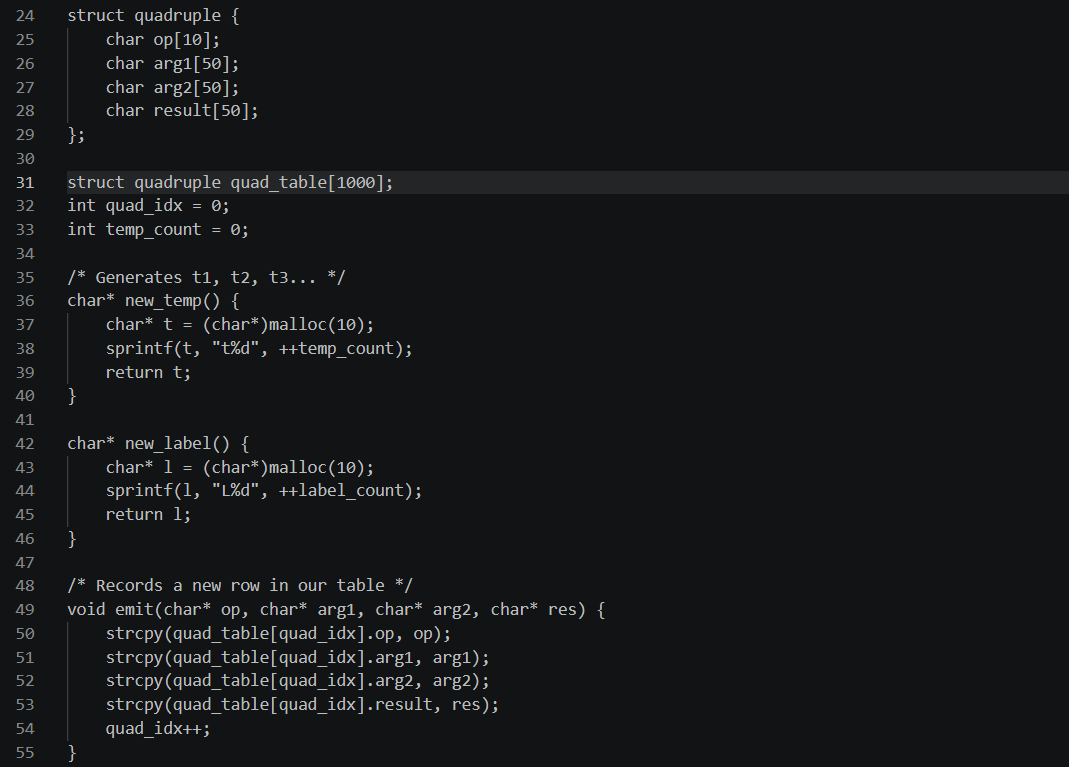
\includegraphics[width=0.9\textwidth]{./Images/image1.png}
    \caption{Quadruple representation and helper routines in \texttt{yapl.y}: global IR table, temporary generator, label generator, and \texttt{emit()} API.}
\end{figure}


\subsection{2. Lexical Value Propagation from Tokens}
\begin{itemize}
    \item \textbf{Implementation details:} Updated identifier and integer-constant rules in \texttt{yapl.l} to copy \texttt{yytext} into \texttt{yylval.name} before returning tokens.
    \item \textbf{How this helps IR generation:} Preserves exact variable names and literal values so emitted TAC contains source-accurate operands.
    \item \textbf{Technical impact:} Parser actions can directly consume identifier and constant text while building quadruples.
    \item \textbf{Why this is necessary:} If token lexemes are not forwarded to parser semantic values, TAC cannot correctly represent program variables and constants.
\end{itemize}

\begin{figure}[H]
    \centering
    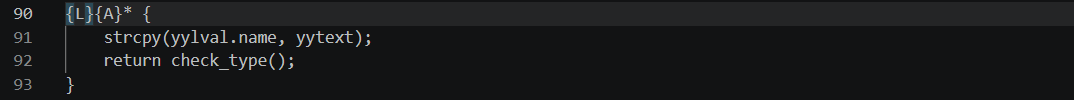
\includegraphics[width=0.45\textwidth]{./Images/image8.png}
    \hfill
    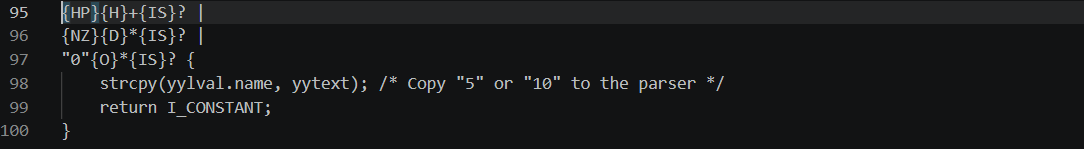
\includegraphics[width=0.45\textwidth]{./Images/image9.png}
    \caption{Lexer updates in \texttt{yapl.l}: identifier and integer lexemes copied into \texttt{yylval.name} for TAC operands.}
\end{figure}

\subsection{3. Semantic Value Flow Across Grammar}
\begin{itemize}
    \item \textbf{Implementation details:} Added \texttt{\%union} with \texttt{name[50]} and assigned \texttt{\%type <name>} to expression-related nonterminals in \texttt{yapl.y}.
    \item \textbf{How this helps IR generation:} Allows each grammar reduction to return either a symbol/literal or a temporary name, enabling parent rules to use child results directly while emitting TAC.
    \item \textbf{Technical impact:} Value propagation works across the full expression chain (primary $\rightarrow$ unary $\rightarrow$ multiplicative $\rightarrow$ additive $\rightarrow$ relational), which is required to emit correct operand references.
    \item \textbf{Why this is necessary:} If nonterminals do not carry semantic names, parent rules lose child computation results and cannot form valid TAC operands.
\end{itemize}

\begin{figure}[H]
    \centering
    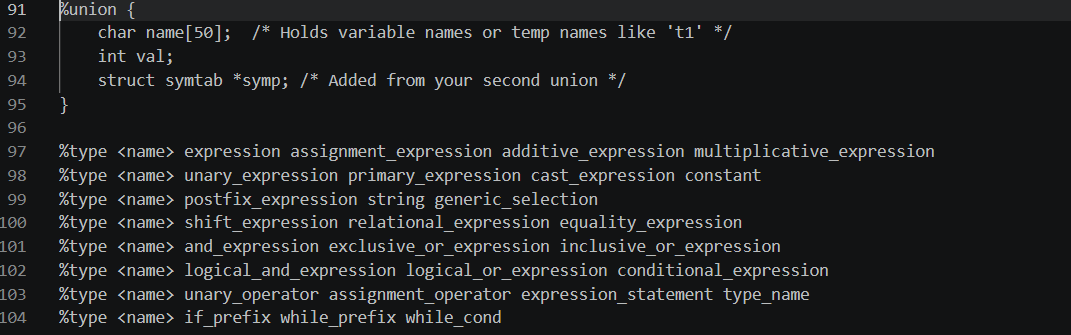
\includegraphics[width=0.9\textwidth]{./Images/image2.png}
    \caption{Semantic value plumbing in \texttt{yapl.y} using \texttt{\%union} and \texttt{\%type <name>} for expression-level TAC propagation.}
\end{figure}

\subsection{4. Expression Evaluation and TAC Emission}
\begin{itemize}
    \item \textbf{Implementation details:} Attached semantic actions to unary, arithmetic, relational, equality, and logical expression rules; each action creates temporaries and calls \texttt{emit()}.
    \item \textbf{How this helps IR generation:} Converts parse-tree computations into explicit TAC steps, where intermediate results are materialized as temporaries and reused in higher-level expressions.
    \item \textbf{Technical impact:} Operator precedence is preserved naturally by grammar structure, and each reduction emits exactly one computation step, making the final quadruple sequence deterministic and debuggable.
    \item \textbf{Example effect:} For \texttt{c = a + b * 5}, multiplication is emitted first into \texttt{t1}, then addition into \texttt{t2}, then assignment \texttt{c = t2}.
\end{itemize}

\begin{figure}[H]
    \centering
    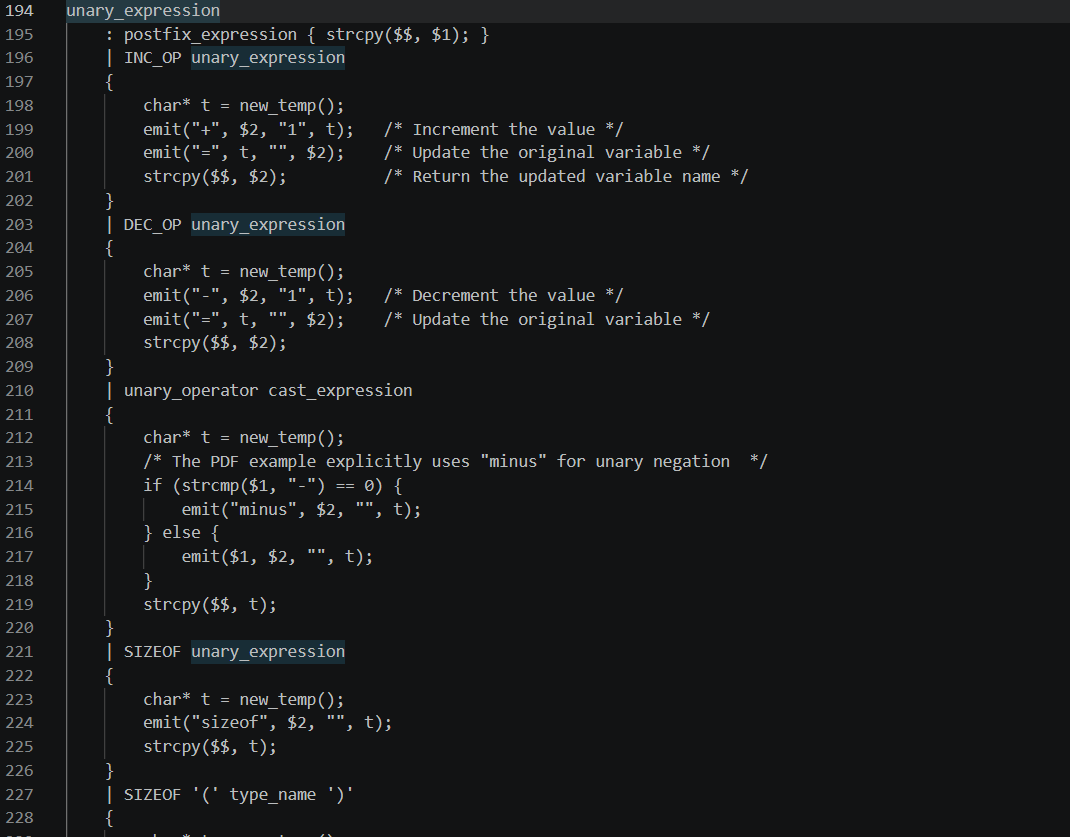
\includegraphics[width=0.9\textwidth]{./Images/image3.png}
    \caption{Expression lowering rules in \texttt{yapl.y}: arithmetic/relational/logical operations emitting TAC with temporaries.}
\end{figure}


\subsection{5. Assignment Handling and LHS Safety}
\begin{itemize}
    \item \textbf{Implementation details:} Enhanced assignment actions to validate the target and force the final \texttt{=} emission to the original LHS identifier.
    \item \textbf{How this helps IR generation:} Preserves assignment semantics (e.g., \texttt{a = E}) by preventing incorrect IR forms where a temporary is mistakenly treated as the final destination.
    \item \textbf{Technical impact:} Handles simple assignment and compound assignment uniformly, and protects against erroneous LHS lowering caused by unary/rewrite side effects.
    \item \textbf{Why this is necessary:} The final store must always target program variables (e.g., \texttt{a}), otherwise generated TAC can become semantically invalid even if parsing succeeds.
\end{itemize}

\begin{figure}[H]
    \centering
    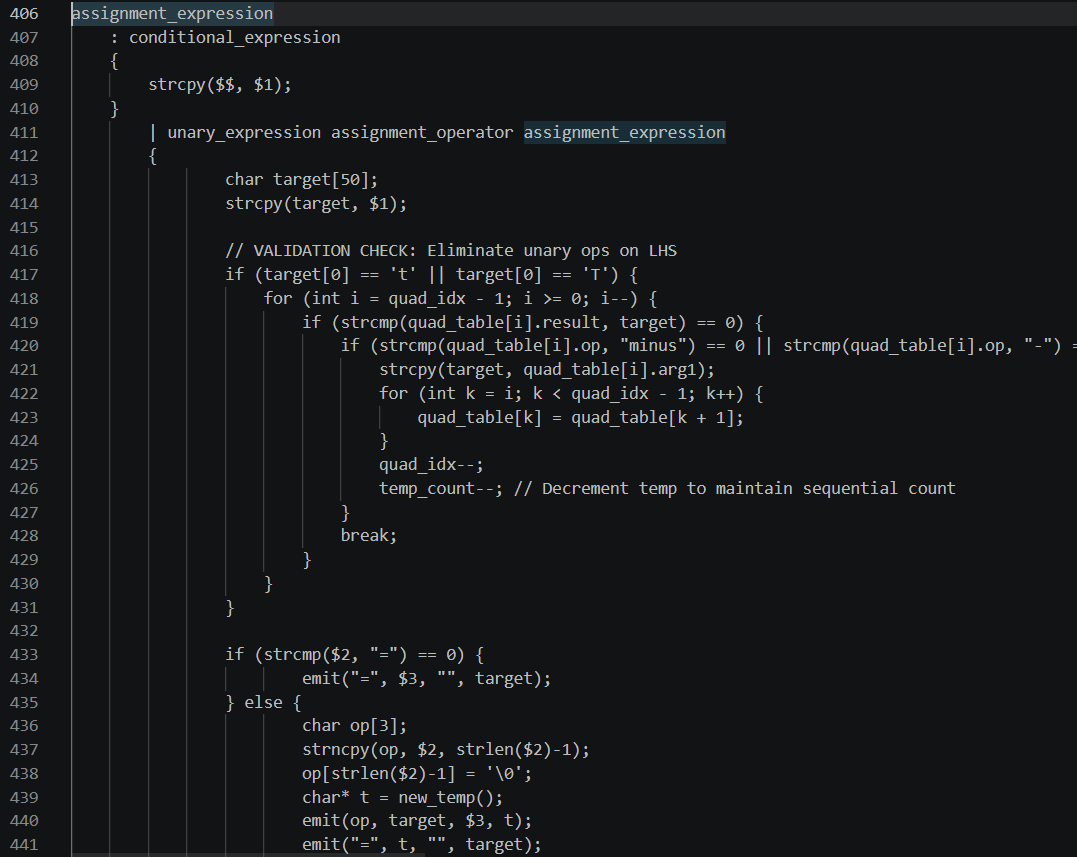
\includegraphics[width=0.9\textwidth]{./Images/image5.png}
    \caption{Assignment translation logic with LHS safety validation to preserve correct final destination in emitted TAC.}
\end{figure}

\subsection{6. Control-Flow Lowering with Labels and Jumps}
\begin{itemize}
    \item \textbf{Implementation details:} Added helper nonterminals and actions for conditionals/loops that emit \texttt{ifFalse}, \texttt{goto}, and \texttt{LABEL} instructions.
    \item \textbf{How this helps IR generation:} Lowers structured control flow into branch-and-label TAC, producing an explicit control-flow graph that can be analyzed or optimized later.
    \item \textbf{Technical impact:} The grammar now emits entry, body, increment, and exit labels for loops and emits true/false branch structure for conditionals, including if-elif-else chains.
    \item \textbf{Why this is necessary:} High-level constructs cannot be consumed by later compiler stages directly; they must be transformed into explicit jump-based flow in IR.
\end{itemize}

\begin{figure}[H]
    \centering
    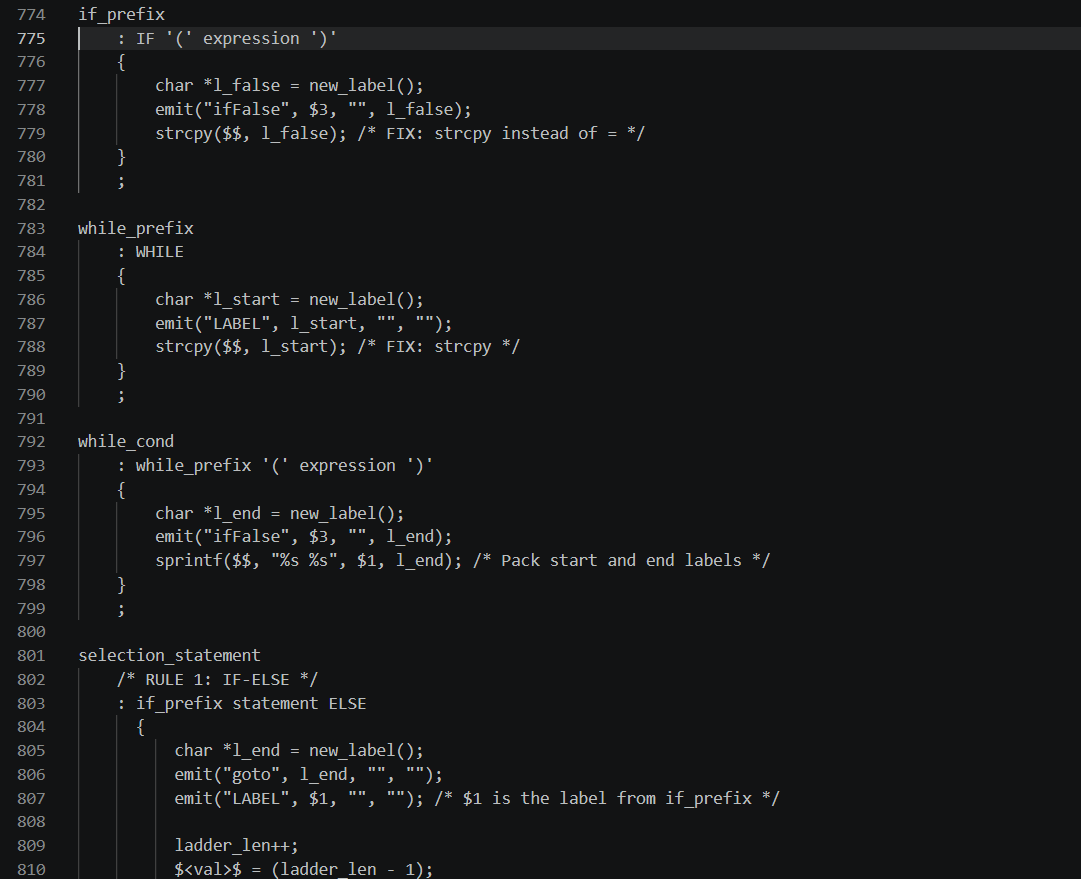
\includegraphics[width=0.9\textwidth]{./Images/image6.png}
    \caption{Control-flow TAC generation for conditionals and loops using \texttt{ifFalse}, \texttt{goto}, and \texttt{LABEL}.}
\end{figure}

\subsection{7. Output and Diagnostics Flow}
\begin{itemize}
    \item \textbf{Implementation details:} Added \texttt{print\_quad\_table()} and updated \texttt{main()} to print source, diagnostics, and generated TAC.
    \item \textbf{How this helps IR generation:} Makes IR output directly visible for validation, helping confirm that semantic actions produce the expected quadruples per testcase.
    \item \textbf{Technical impact:} The output order now clearly mirrors the compilation pipeline: input program $\rightarrow$ parser success and counters $\rightarrow$ TAC table $\rightarrow$ reverse derivation.
    \item \textbf{Why this is necessary:} Assignment evaluation requires demonstrable generated IR, and this output format provides direct evidence for correctness.
\end{itemize}

\begin{figure}[H]
    \centering
    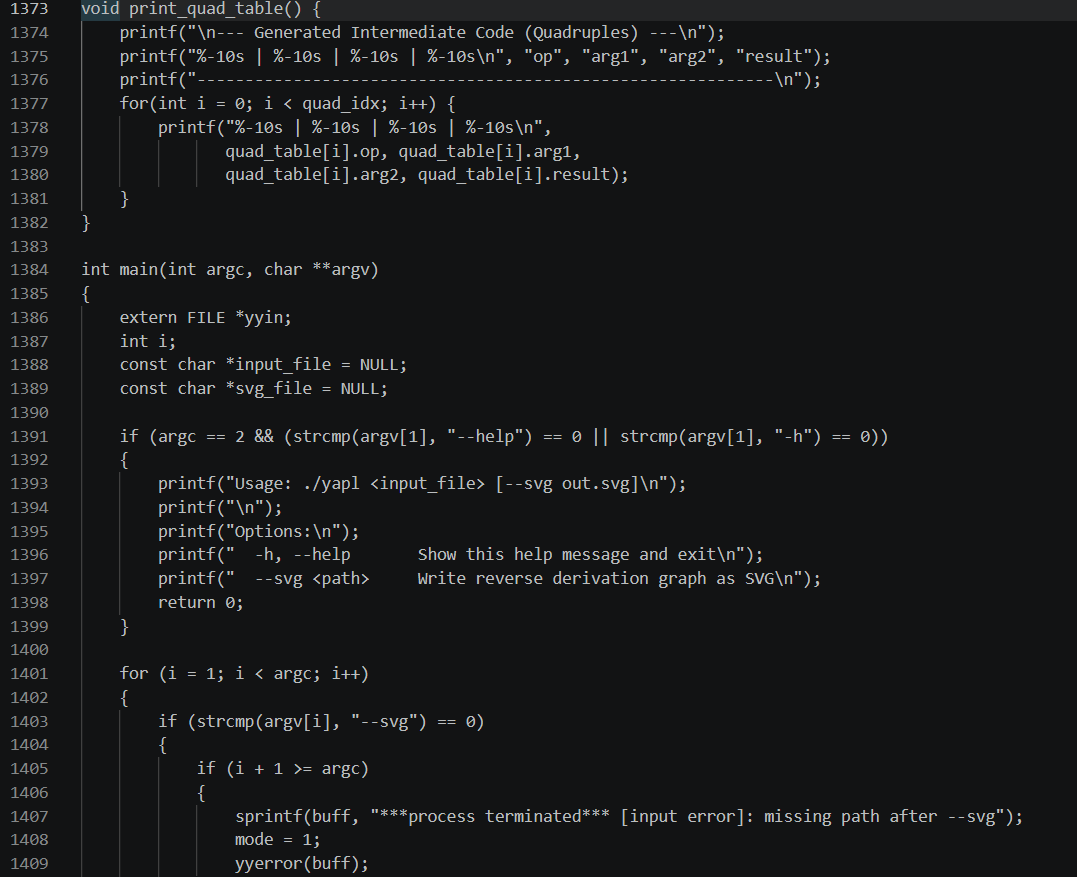
\includegraphics[width=0.9\textwidth]{./Images/image7.png}
    \caption{Driver-side reporting in \texttt{main()}: source echo, parser diagnostics, and tabular quadruple output.}
\end{figure}

Error reporting remains robust through verbose parser diagnostics and guarded input handling, ensuring malformed inputs terminate cleanly with meaningful messages rather than causing unstable behavior.

\section{Part 3 (3 marks): Code Output Format}

This section demonstrates output-format compliance using testcase \texttt{testcases\_a4/tc1.c}.

\subsection{Chosen Testcase}
\begin{lstlisting}
int main() {
    int a; int b; int c;
    a = 10;
    b = 20;
    c = a + b * 5;
}
\end{lstlisting}

\subsection{Observed Generated IR (from tool output)}
\begin{lstlisting}
op         | arg1       | arg2       | result
------------------------------------------------------------
=          | 10         |            | a
=          | 20         |            | b
*          | b          | 5          | t1
+          | a          | t1         | t2
=          | t2         |            | c
\end{lstlisting}

\subsection{Requirement-wise Explanation}
\begin{enumerate}
    \item \textbf{Intermediate code printed row-by-row from top to bottom:} The IR appears in execution order. First constants are assigned to \texttt{a} and \texttt{b}, then multiplication is emitted, then addition, and finally assignment to \texttt{c}. This matches top-down TAC generation.
    \item \textbf{Readable temporary variable naming (\texttt{t1}, \texttt{t2}, ...):} Intermediate values are stored in \texttt{t1} and \texttt{t2}, making data flow easy to follow.
    \item \textbf{Clear source code and IR separation:} Output prints source under the input-program header and prints TAC under the generated-intermediate-code header, so both phases are clearly separated.
\end{enumerate}

\subsection{Result}
The implementation satisfies all three Part 3 requirements. The generated output is tabular, ordered, and readable, which supports both debugging and evaluation.


\begin{figure}[H]
    \centering
    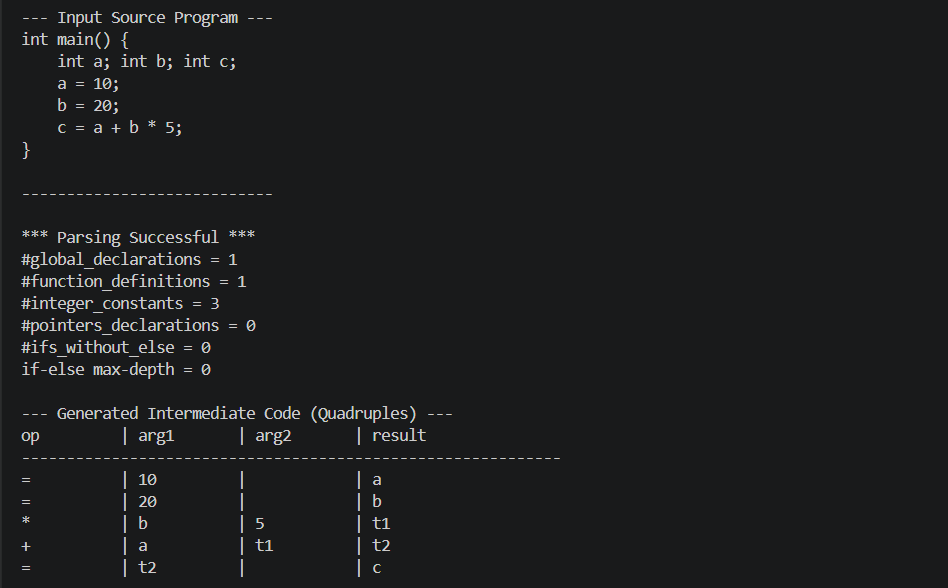
\includegraphics[width=0.9\textwidth]{./Images/image10.png}
    \caption{row-wise TAC table with readable temporaries and separated source/IR blocks.}
\end{figure}


\section{Part 4 (3 marks): Error Handling}

This section explains diagnostic behavior during code generation and parsing.

\subsection{Observed Error Behavior (invalid-input run)}
To verify robustness on incorrect input, the parser was run on:
\begin{lstlisting}
int main() {
    int a;
    a = b + ;
    return 0;
}
\end{lstlisting}

Observed diagnostic:
\begin{lstlisting}
***parsing terminated*** [syntax error]
line 3, column 13: unexpected token ";"
\end{lstlisting}

\subsection{Requirement-wise Explanation}
\begin{itemize}
    \item \textbf{Detect invalid expressions or unsupported constructs:} The malformed assignment \texttt{a = b + ;} is detected immediately and parser termination is triggered correctly.
    \item \textbf{Display meaningful error messages:} The diagnostic includes both line and column information and reports the unexpected token, which is useful for debugging.
    \item \textbf{Ensure program does not crash on incorrect input:} The parser exits gracefully with a controlled error message instead of crashing or producing corrupted IR.
\end{itemize}

\subsection{Result}
The implementation satisfies Part 4 expectations for practical diagnostics and runtime robustness. Invalid input is handled predictably and reported with useful location information.


\begin{figure}[H]
    \centering
    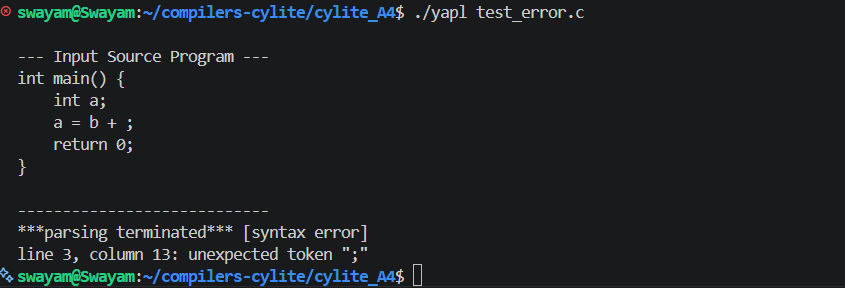
\includegraphics[width=0.9\textwidth]{./Images/image11.png}
    \caption{meaningful syntax-error reporting and graceful termination on incorrect input.}
\end{figure}


\section{Build and Reproduction Steps}

\begin{lstlisting}
cd cylite_A4
make clean
make
./yapl testcases_a4/tc1.c
\end{lstlisting}



\section{Conclusion}

Assignment 4 successfully transforms CYLite into a working intermediate code generator using TAC quadruples. Compared to Assignment 3, the parser now carries semantic values and emits executable IR for expressions and control flow, while preserving detailed diagnostics and stable behavior on invalid input.

The implementation demonstrates end-to-end translation from grammar reductions to structured quadruple output with labels, temporaries, and branch instructions. This establishes a clean base for subsequent compiler phases such as optimization and target code generation.

\end{document}
